\documentclass[a4paper, ngerman]{article}
\usepackage[ngerman]{babel}
\usepackage[ngerman]{isodate}
%\usepackage[T1]{fontenc}
%\usepackage{selinput} 
\usepackage[utf8]{inputenc}
\usepackage{parskip}
\usepackage{csquotes}
\usepackage{booktabs}
\usepackage{amsmath}
\usepackage{graphicx}
\usepackage{tikz}
\usepackage{pgfplots}
\usepackage{fancyhdr}
\usepackage{titling}
\usepackage{lastpage}
\usepackage{tabularx}
\usepackage[Q=yes]{examplep}
\usepackage[toc,page]{appendix}
\usepackage{a4wide}
\usepackage{multirow}
\usepackage{framed}
\usepackage{graphicx}
\usepackage{float}


\renewcommand{\headrulewidth}{1pt}
\renewcommand{\footrulewidth}{1pt}
% \renewcommand{\familydefault}{\sfdefault}


\pagestyle{fancy}
\fancyhf{}

\rhead{Kapeller}
\lhead{Physik}
\lfoot{\origdate\today}
\rfoot{Seite \thepage\ von \pageref{LastPage}}

\begin{document}

\section*{Zusammenfassung Kapitel 3: Wellen und Teilchen}
\subsection*{Licht im Interferometer}
Photonen verhalten sich unter gewissen Umständen wie Wellen und unter anderen Umständen wie Teilchen $\rightarrow$ \textbf{Wellen-Teilchen-Dualismus}. Ein Merkmal
des Wellenverhaltens ist die \textbf{Interferenz}. Bei folgendem Experiment steht dies im Vordergrund.
\subsubsection*{Experiment: Interferometer}

\begin{figure}[H]
    \centering
    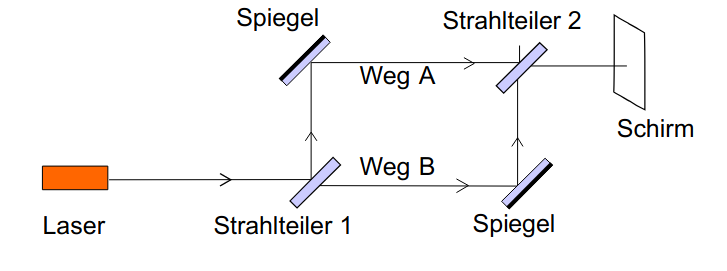
\includegraphics[scale=0.5]{Interferometer.png}
    \caption{Interferometer}
\end{figure}

Zuerst wird das Licht im ersten Strahlenteiler in zwei Strahlen (Weg A, Web B) aufgespalten.
Danach werden sie im zweiten Strahler wieder zusammengeführt. Der wichtige Aspekt dabei ist, dass
es einen Gangunterschied zwischen den beiden Strahlen gibt, der zu einer Interferenz bei der Zusammenführung führt.
Diese Interferenzen ergeben ein \textbf{Interferenzmuster}.

Dieses Experiment bestätigt die Wellentheorie. Würde man das selbe Experiment mit einzelnen Photonen durchführen können,
könnte man möglicherweise sowohl Wellen- als auch Teilcheneigenschaften beobachten.

\subsection*{Vom Lichtstrahl zu einzelnen Photonen}
Um von Welle zu einzelnem Photonen kommen $\rightarrow$ Licht $"$verdünnen$"$.
\subsubsection*{Experiment}
Es wird durch mehrere Graufilter das Licht verdünnt. Dadurch wird die Intensität stark verringert, aber
einzelnen Photonen kann man mit dem menschlichen Auge nicht erkennen. Deshalb werden CCD-Elemente verwendend, die
die einzelnen Photonen registrieren können.

Dieses Verfahren ist die Grundlage aller Experimente mit einzelnen Photonen.

\subsection*{Interferometrie mit einzelnen Photonen}
\subsubsection*{Experiment}
In der Computersimulation kann dasselbe Interferometer-Experiment auch mit einzelnen Photonen gestartet werden.
Dadurch entsteht nicht sofort das gesamte Muster, sondern mit jedem Photon ein einzelner Punkt, der am Schluss zu dem Muster führt. \\
$\rightarrow$ \textbf{Dualismus von Welle und Teilchen}: jedes Photon übertragt seine gesamte Energie auf einen Punkt, die Welle $"$dehnt$"$
ihre Energie auf das gesamte Muster.

\end{document}